\documentclass[14pt,a4paper,fleqn]{extarticle}
\usepackage[T2A,T1]{fontenc}
\usepackage[utf8]{inputenc}
\usepackage[russian]{babel}
\usepackage{amsmath}
\usepackage{graphicx}
\usepackage{tabularx}
\usepackage{boldline}
\usepackage{makecell}
\usepackage{arydshln}
\usepackage{mathtools}

\graphicspath{ {./images/} }
\setlength{\mathindent}{0pt}
\setlength\parindent{0pt}


\begin{document}
	\begin{titlepage}
		
\includegraphics[scale=0.12]{logo}
		\begin{center}
			\textbf{МИНОБРНАУКИ РОССИИ}\\
			\vspace{0.2cm}
			\textbf{Федеральное государственное бюджетное образовательное учреждение высшего образования}\\
			\textbf{«САНКТ-ПЕТЕРБУРГСКИЙ ГОСУДАРСТВЕННЫЙ ЭКОНОМИЧЕСКИЙ УНИВЕРСИТЕТ»}\\
			\vspace{0.6cm}
			Факультет информатики и прикладной математики\\
			Кафедра прикладной математики и экономико-математических методов\\
			\vspace{1cm}
			\textbf{ОТЧЁТ}\\
			по дисциплине:\\
			\textbf{«Методы оптимизации»}\\
			на тему:\\
			\textbf{«Решение транспортной задачи по критерию времени. Задание 9»}\\
		\end{center}
		\vspace{1cm}
		Направление: 01.03.02\\
		Обучающийся: Бронников Егор Игоревич\\
		Группа: ПМ-1901\\
		\vfill
		\begin{center}
			Санкт-Петербург\\
			2021\\
		\end{center}
	\end{titlepage}
\section*{Задача 1}
\subsection*{a. Метод минимального элемента}
\begin{center}
	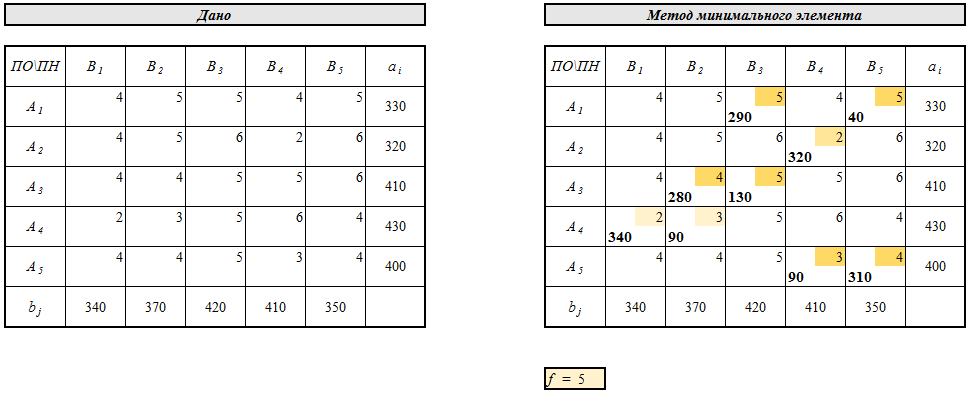
\includegraphics[scale=0.51]{1}
\end{center}
\small Рассмотрим начальный план, полученный методом минимального элемента.\\
На 1 итерации попробуем избавиться от клетки $A_1B_5$.
\begin{center}
	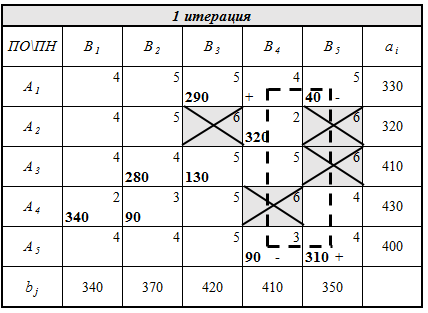
\includegraphics[scale=0.64]{2}
\end{center}
Запрещаем все клетки большие 5. Строим цикл: $A_1B_4 \rightarrow A_1B_5 \rightarrow A_5B_5 \rightarrow A_5B_4$.\\
Таким образом, клетка $A_1B_4$ стала базисной, а клетка $A_1B_5$ стала свободной.
\newpage
На 2 итерации уже не получается построить цикл, чтобы избавиться от клеток $A_1B_3$ и $A_3B_3$.
\begin{center}
	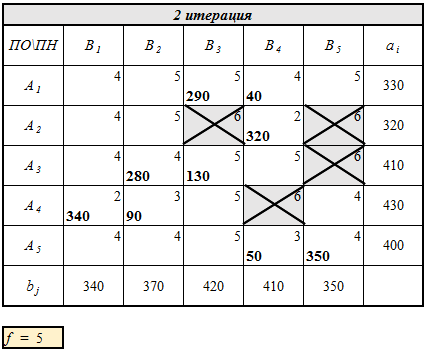
\includegraphics[scale=0.64]{3}
\end{center}
Таким образом, значение целевой функции: $f = max \hspace*{0.1cm} \{5,4,2,4,5,2,3,3,4\} = 5$.
\newpage
\subsection*{b. Метод северо-западного угла}
\begin{center}
	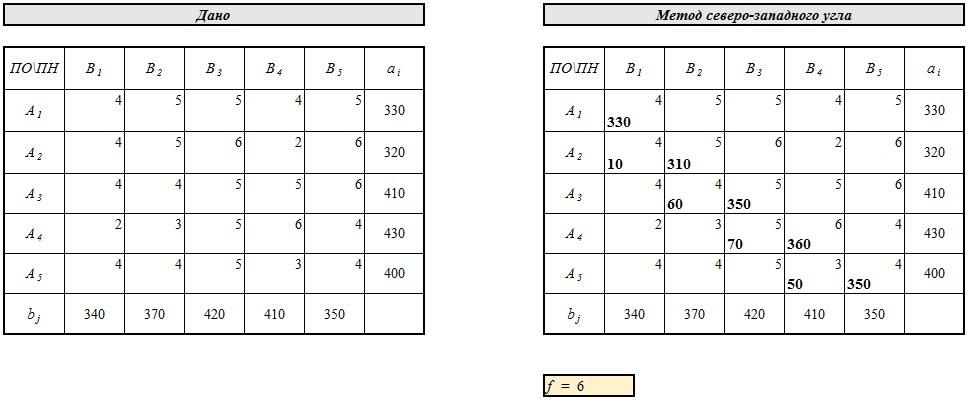
\includegraphics[scale=0.51]{4}
\end{center}
Рассмотрим начальный план, полученный методом северо-западного угла.\\
На 1 итерации попробуем избавиться от клетки $A_4B_4$.
\begin{center}
	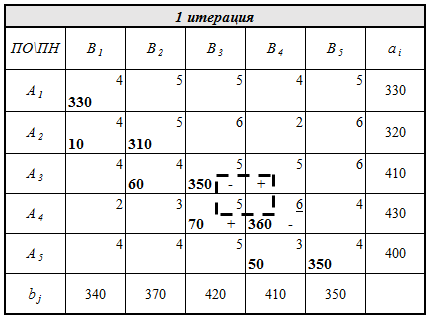
\includegraphics[scale=0.64]{5}
\end{center}
Запрещаем все клетки большие 6. Строим цикл: $A_3B_4 \rightarrow A_3B_3 \rightarrow A_4B_3 \rightarrow A_4B_4$.\\
Таким образом, мы сделали перевозку в клетке $A_4B_4$ меньше на 350 единиц.
\newpage
На 2 итерации добиваем клетку $A_4B_4$.
\begin{center}
	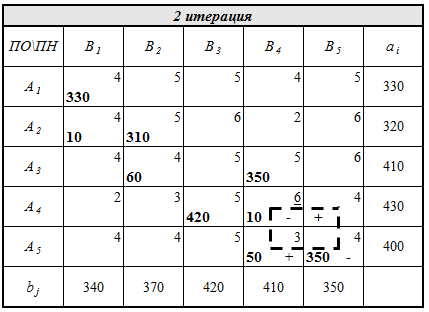
\includegraphics[scale=0.64]{6}
\end{center}
Запрещаем все клетки большие 6. Строим цикл: $A_4B_5 \rightarrow A_4B_4 \rightarrow A_5B_4 \rightarrow A_5B_5$.\\
Таким образом, клетка $A_4B_5$ стала базисной, а клетка $A_4B_4$ стала свободной.\\\\
На 3 итерации уже не получается построить цикл, чтобы избавиться от клеток $A_3B_4$ и $A_2B_2$.
\begin{center}
	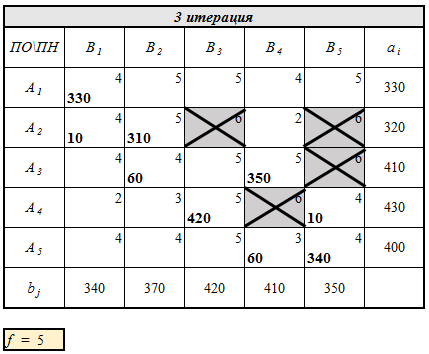
\includegraphics[scale=0.64]{7}
\end{center}
Таким образом, значение целевой функции: $f = max \hspace*{0.1cm} \{4,4,5,4,5,5,4,3,4\} = 5$.
\newpage
\section*{Задача 2}
\begin{center}
	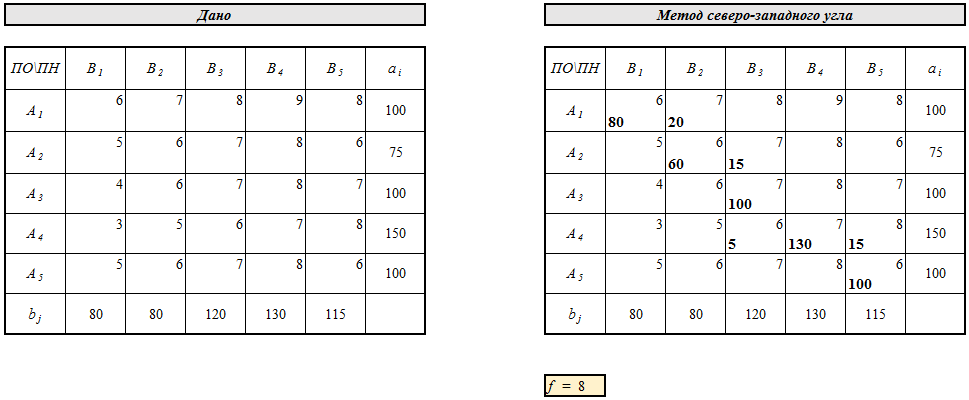
\includegraphics[scale=0.51]{8}
\end{center}
Рассмотрим начальный план, полученный методом северо-западного угла.\\
На 1 итерации попробуем избавиться от клетки $A_4B_5$.
\begin{center}
	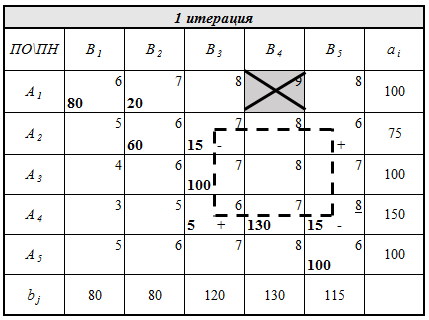
\includegraphics[scale=0.64]{9}
\end{center}
Запрещаем все клетки большие 8. Строим цикл: $A_2B_5 \rightarrow A_2B_3 \rightarrow A_4B_3 \rightarrow A_4B_5$.\\
Таким образом, клетка $A_4B_5$ стала базисной, а клетка $A_2B_5$ стала свободной.
\newpage
На 2 итерации уже не получается построить цикл, чтобы избавиться от клеток $A_1B_2$, $A_4B_4$ и $A_3B_3$.
\begin{center}
	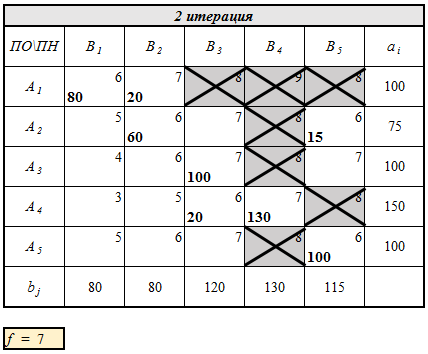
\includegraphics[scale=0.64]{10}
\end{center}
Таким образом, значение целевой функции: $f = max \hspace*{0.1cm} \{6,7,6,7,6,7,6,6\} = 7$.
\end{document}